\documentclass[wmii,inf,mgr]{uwmthesis}
\usepackage{graphicx}
\graphicspath{ {images/} }
\usepackage[MeX]{polski}
\usepackage[utf8]{inputenc}
\usepackage{url}


\date{2017}
\title{Prezentacja rozkładu Mostu Obrotowego w Giżycku z wykorzystaniem interaktywnych tablic LED}
\author{Maciej Czajkowski}
\etitle{Presentation of the distribution of the Swing Bridge in Giżycko using interactive LED arrays}
\wykonanaw{katedrze Metod Matematycznych Informatyki}
\ewykonanaw{Chair of Mathematical Methods of Informatics}

\podkierunkiem{dr Krzysztofa Sopyły}
\epodkierunkiem{dr Krzysztof Sopyła}

\begin{document}
	
\maketitle
	
\tableofcontents

\chapter*{Wstęp}
\section{Most Obrotowy w Giżycku}
	Most Obrotowy w Giżycku znajdujący się nad Kanałem Giżyckim przy zbiegu ulic Olsztyńskiej, Stanisława Moniuszki i Nadbrzeżnej to jeden z pięciu mostów rozpiętych nad kanałem. Jest to niewątpliwie jeden z tutejszych najciekawszych zabytków, ponieważ działających mostów takiej konstrukcji w Europie jest zaledwie kilka. \par
	Sezon letni to czas zwiększonego zainteresowania mostem turystów chętnych obejrzenia i udokumentowania chwili zmiany stanu mostu. Wartym wspomnienia jest fakt, że samo przęsło mostu waży ponad 100 ton, a obecnie - i tak, jak w momencie oddania do użytku - obsługiwany jest przez jedną osobę. Dróżnik obraca mostem ręcznie. Giżycki zabytek został zbudowany w 1898 roku przez firmę Beuchelt& Co. Grünbergi.Schl. z Zielonej Góry, żeby zapewnić dojazd z miasta do znajdującej się po zachodniej stronie kanału Twierdzy Boyen\footnote{http://bit.ly/2keuPD3 [dostęp styczeń 2017]}. W latach 60-tych XX wieku, most został zmodernizowany i uzyskał napęd elektryczny. Jednak zastosowanie nowej techniki okazało się być tragiczne w skutkach dla nadbrzeża, w które most uderzał przy każdym otwarciu. Na prośbę mieszkańców Most został rozebrany a jego miejsce zajął tymczasowy most wojskowy, który nie tylko nie wpisywał się w architekturę Giżycka, ale także był krytykowany przez samych Giżycczan. \par
	W 1993 roku po generalnym remoncie oryginalny most (już bez napędu elektrycznego) przywrócono do pracy i do dnia dzisiejszego działa on bez zarzutu, jest dumą i wizytówką Giżycka i jego władz. \par
\begin{figure}[h]
\centering
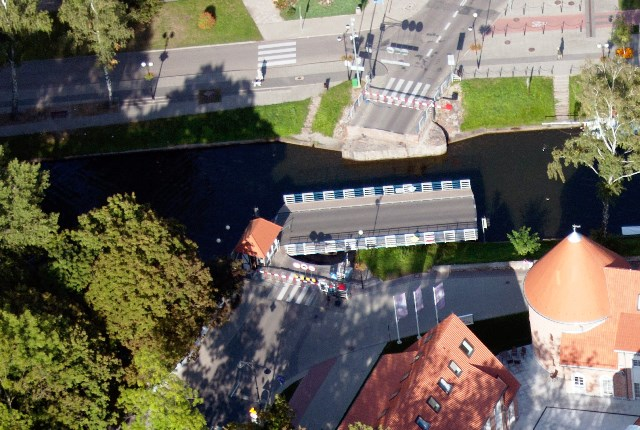
\includegraphics[width=0.5\textwidth]{obraz1}
\caption{Most Obrotowy z lotu ptaka [ źródło: http://bit.ly/2jqkQGB ]}
\end{figure}

\section{Cel pracy}
	Celem niniejszej pracy magisterskiej jest opracowanie sposobu prezentacji rozkładu Mostu Obrotowego w Giżycku na interaktywnych tablicach wykonanych w technologii LED ustawionych na terenie miasta oraz budowa własnego rozwiązania opartego o mikrokomputer Raspberry Pi jako kontrolera.\par
	Dwa lata temu w głosowaniu na giżycki budżet partycypacyjny został wyłoniony projekt systemu zegara odliczającego czas do zmiany stanu mostu z otwartego na zamknięty i odwrotnie. Autor projektu użył sformułowań "zaprojektować i wdrożyć" pozostawiając wszelkie założenia projektowe w rękach ludzi z Urzędu Miasta. Moim pomysłem było połączenie powstającego systemu tablic z istniejącym już i całkiem dobrze rozwiniętym systemem aplikacji \textbf{"Most Obrotowy na Androida"}. \par
	Został wybrany polski producent oferujący technologię live streamingu\footnote{http://bit.ly/2kf55qr [dostep styczeń 2017]} oraz zakupione zostały dwie pierwsze tablice stanowiące szkielet budowanej sieci (obie znalazły miejsce przy Moście Obrotowym). W oparciu o biblioteki producenta napisałem w języku C\# aplikację sterującą, jednak z niewyjaśnionych przyczyn tablice się zawieszają w losowych odstępach czasu. Stąd też pomysł opracowania i wdrożenia własnego rozwiązania dającego pełną kontrolę nad sterowaniem, a co za tym idzie, samą tablicą.
\begin{figure}[h]
\centering
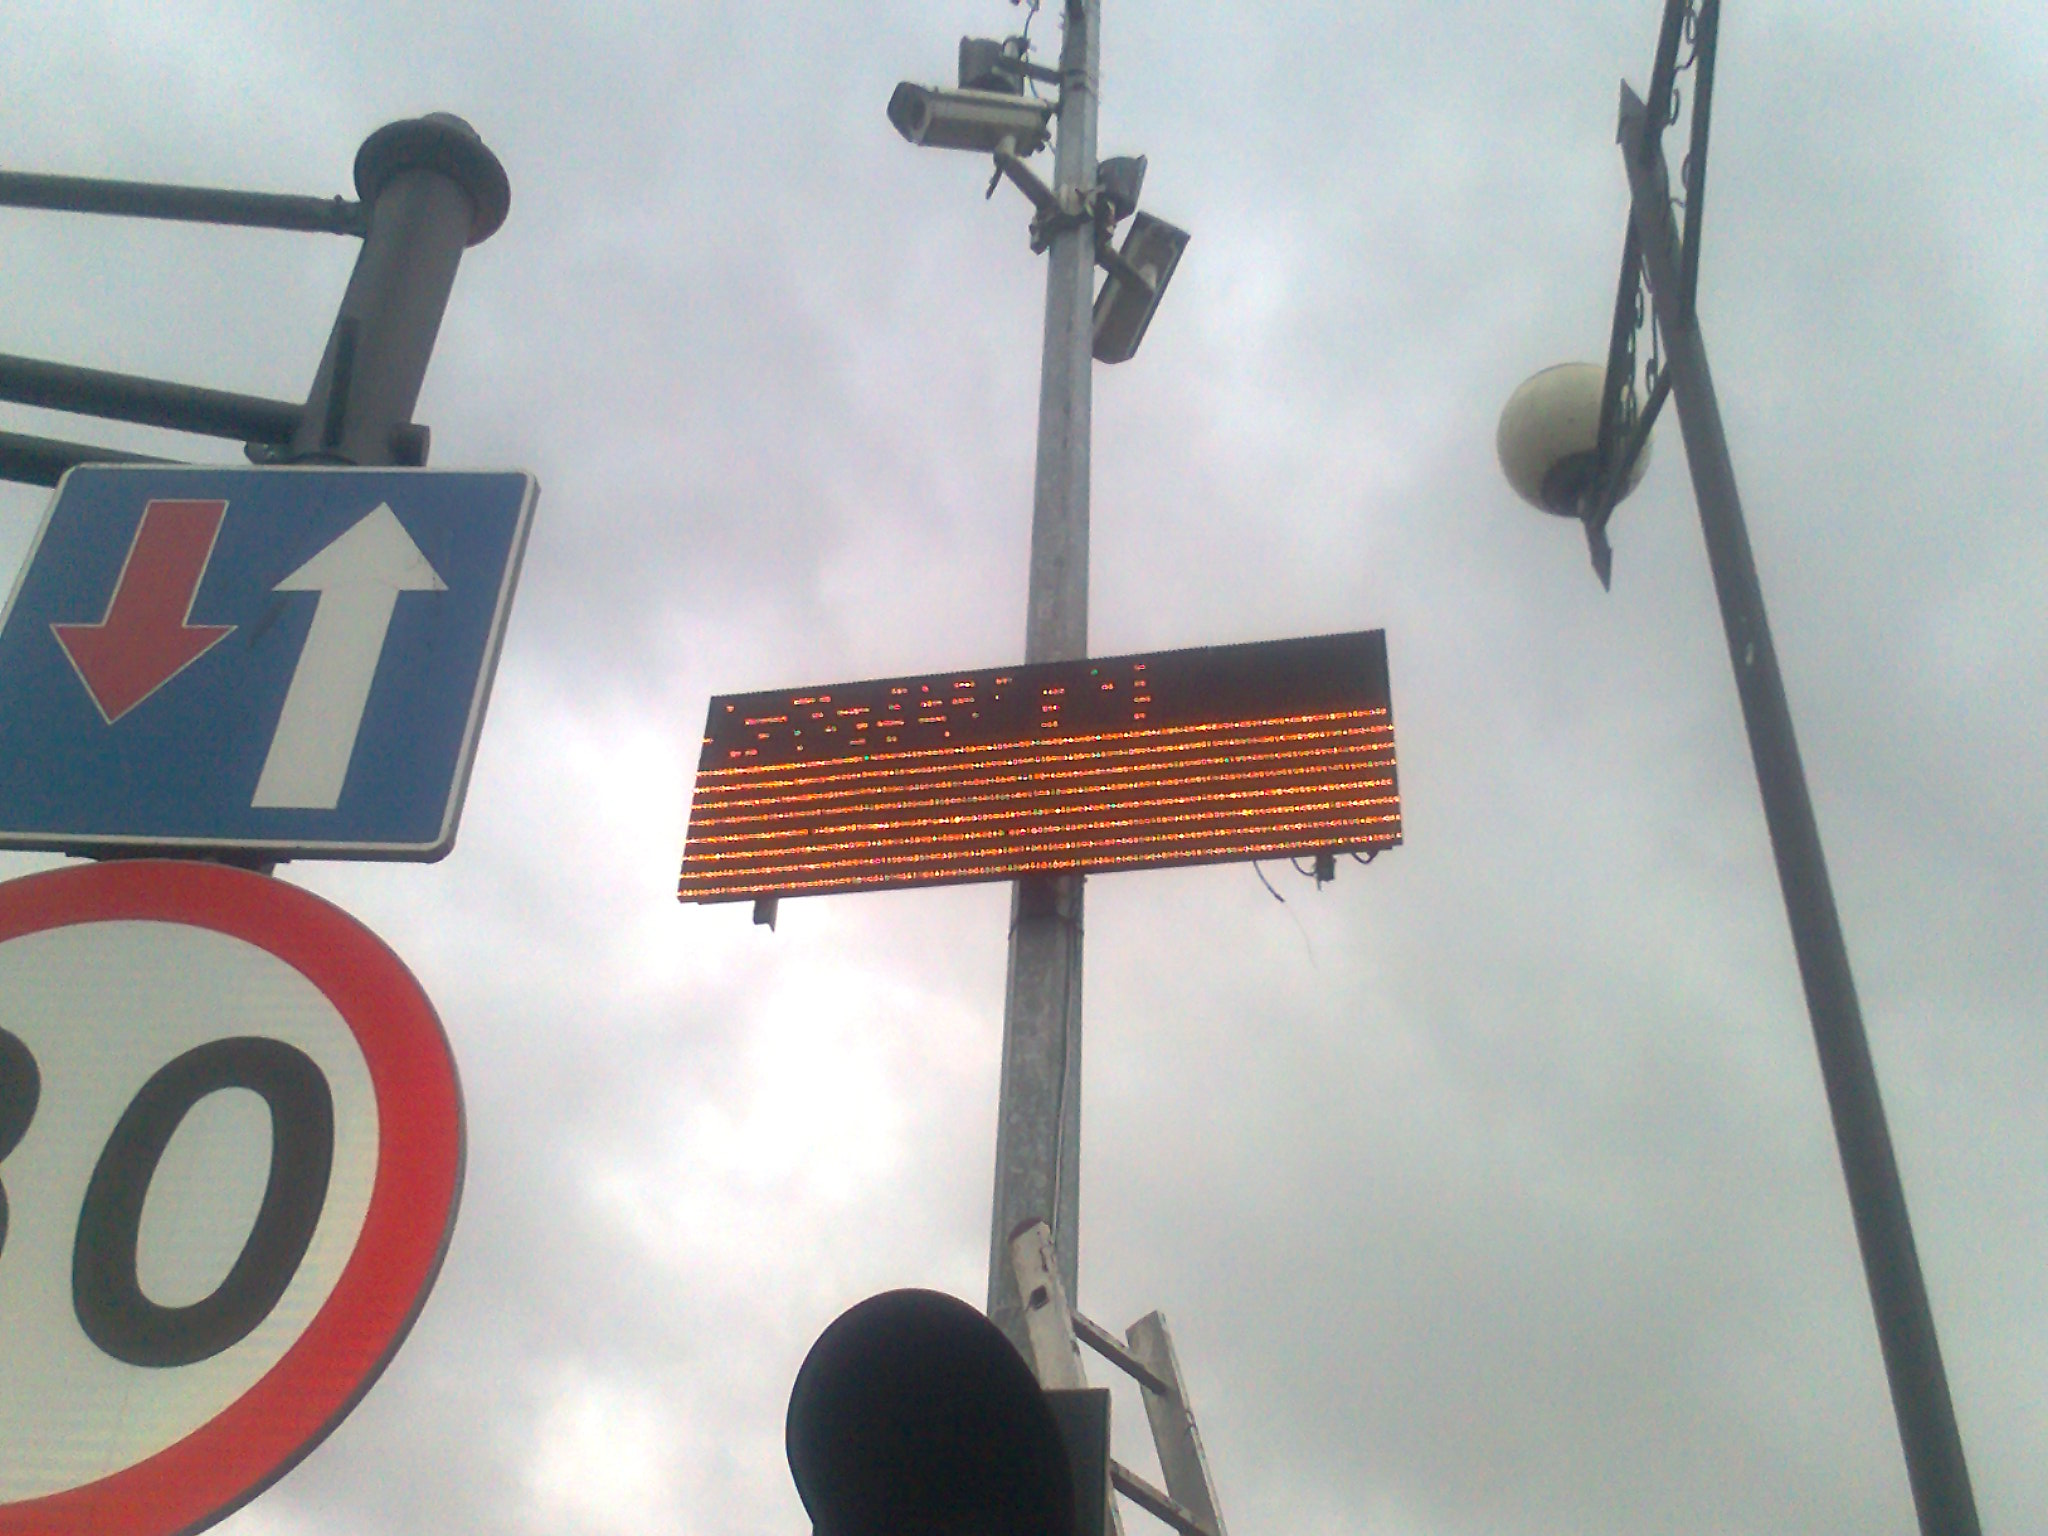
\includegraphics[width=0.5\textwidth]{obraz2}
\caption{Tablica nie odpowiada na polecenia [źródło: materiały własne]}
\end{figure}

\section{Zakres pracy}
	Domyślnie aplikacja ma działać na mikrokomputerze Raspberry Pi. Opracowanie własnego rozwiązania ma na celu wyeliminowanie błędów i problemów obecnej wersji systemu. Przede wszystkim projekt musi usprawnić komunikację między administratorem a tablicami oraz zniwelować opóźnienia w transmisji danych w obecnej metodzie komunikacyjnej. Na polecenie zastępcy Burmistrza Giżycka większość tablic odbierać dane będzie poprzez sieć komórkową. Taka decyzja wynika z faktu, że nie w każdym miejscu da się doprowadzić stałe łącze lub koszty przyłącza są nieadekwatne do kosztów całego projektu. \newpage 
	Planowany zakres zagadnień:
	
\begin{itemize}
	\item opis obecnego systemu, wykorzystanych technologii, aplikacji sterującej
	\item realizacja spójności systemu
	\item rozpoznanie się w elementach budowy interaktywnej tablicy LED
	\item opracowanie schematu połączenia i sterowania
	\item dostosowanie protokołu HUB75 (tablica RGB) do protokołu HUB12 (tablica mono)
	\item testy opracowywanego schematu tablicy
	\item program sterujący zgodny z architekturą Raspberry Pi
	\item integracja z obecnym systemem i zachowanie maksymalnie możliwej spójności
	\item projekt i wdrożenie aplikacji sterującej parametrami tablicy takimi jak np. jasność
\end{itemize}




\chapter{Opis problemu}
Curabitur congue rutrum justo nec ultrices. Ut orci lacus, dignissim sed facilisis non, dictum eu lectus. Suspendisse potenti. Nulla commodo et ex eu commodo. Integer sit amet leo tincidunt, pharetra sem sed, interdum diam.
\section{Proponowane rozwiązanie}
\section{Wykorzystane technologie}
\subsection{C-sharp}
\section{Sekcja 3}

\chapter{Budowa stanowisk}
\chapter{Projekt systemu}
(użyte materiały etc)
\section{Połączenia}
\section{Przekaźniki}
\section{Sekcja 3}

\chapter{Implementacja}

Aliquam non erat cursus, malesuada tortor sit amet, porttitor dui. Cras iaculis neque at metus viverra, vel rhoncus arcu sollicitudin.
\section{Sprzęt (Raspberry Pi)}
\section{Sekcja 2}
\section{Sekcja 3}
\chapter{Instrukcja uruchomienia}
\chapter{Podsumowanie}
\chapter*{Bibliografia}

\end{document}